\chapter*{Statistics 6}

\newpage
\section{Experimental Design}

    \newpage
    \subsection{Experimental Design}
        \paragraph{Experimental error}
        Experimental error is the effect of other factors other that those controlled by the experimenter. The standard deviation is one way of measuring the experimental error, since its a measure of the spread of data. To minimize experimental error all factors that are not being investigated should be kept constant and a good experiment design should be used.

        \paragraph{Experimental design}
        The simplest experimental design is a paired comparision were experimental error is reduced bu applying the same treatment to the same subjects or in the same condition i.e. testing two diffrent diets on identical twins thus reducing experimental error due to phcological and biological effects.

        \paragraph{Randomisation}
        The purpose of randomisation is to reduce bias. Were possible the experimenter should remove all likely sources of bias by using random sampling to select an unbiased sample and random processes whenever their is a choise such as which twin is assigned which diet. 

        \paragraph{Blocking}
        Completly randomised design is the process of randomly assigning subjects to treatments and uses one-factor analysis of varience. Randomised block design is the process of spliting subjects in to simular subgroups then randomly assigning those in a subgroups to a treatment. This design is analysed using two factor analysis of variance. Randomised block design is used when another factor (a blocking factor) is thought to an effect on the results. 

        \begin{example}
            {
                In a comparision of the drying times of three different types of wood preservatives A, B and C, samples of each four diffrent woods are availible, W1, W2, W3 and W4. Three experimental designs are suggested.
                \begin{center}
                \begin{tabular}{ccc|ccc|ccc}
                & Design 1 & & & Design 2 & & & Design 3 & \\
                A & B & C & A & B & C & A & B & C \\
                \hline
                W1 & W2 & W3 & W1 & W2 & W1 & W1 & W2 & W3 \\
                W1 & W2 & W3 & W2 & W3 & W3 & W3 & W4 & W2 \\
                W1 & W2 & W3 & W3 & W1 & W2 & W4 & W1 & W4 \\
                &    &    & W4 & W4 & W4 & W2 & W3 & W1 \\
                &    &    & W1 & W2 & W3 &    &    &    \\
                \end{tabular}
                \end{center}
            }

            \begin{step}{State two dissadvantages of design 1}
            \begin{itemize}
            \item Each type of preservative is used on only on type of wood thus it would not be possible to tell if any diffrence found was due to diffrent wood or the preservative (or both).
            \item Wood 4 is not included in the test.
            \end{itemize}
            \end{step}

            \begin{step}{Write down the name of design 3}
            Randomised block design
            \end{step}

            \begin{step}{Name the tecnique used to analyse the results from design 3}
            Two factor analysis of varience
            \end{step}

            \begin{step}{State one advantage of design 3 over design 2}
            Design 2 uses some wood samples multiple times whereas design 3 uses all the samples only once. The comparision for mean drying times may be effected in design 2 by the cobination of wood samples used with each preservative.
            \end{step}

            \begin{step}{Explain how randomisation might be used in the context of design 1, 2 and 3}
            \textbf{Design 1} Allocation of wood to treatment should be carried out by a random process, ensuring the results would not be rigged by selecting a wood for the mosted favored preservative.
            
            \textbf{Design 2} A random process would decide which wood was W1 etc, thus the wood used twice would be selected randomly.

            \textbf{Design 3} Less likely to be effected by bias but the order of carrying out treatments should ideally be determined by a random process. 
            \end{step}
        \end{example}

        \paragraph{Control group}
        If a new treatment is applied to an exprimental group, a control group, which recieves no treatment is needed to measure the effects of the new treatment. This control group should as simular as possible to the exprimental group in order to minimize bias.

        \paragraph{Blind trials}
        The plecbo effect is a well known effect were patients will improve by taking a plecbo drug, a treatment which contains no active ingredient. To show that a new drug is effective many more patients must show improvment than those taking the placbo pill. In a blind trial subjects do not know if they are receiving the treatment or the placbo which help reduce bias from the plecbo effect. 
        
        \paragraph{Double blind trials} Doctors that know a patient is on the active drug may expect patients fare better which may be transmitted onto the patient. A double blind trial is were the subject and the person administrating the treatment knows wether a placebo or active drug was given.

        \paragraph{Triple blind trials} To prevent the bias in the statistical analysis it has been suggested that the statician should also not know which patients took the drug which would be a triple blind trial.

        \begin{example}
        {
            To measure the effectiveness of a drug to relive breathlessness 12 subjects, all susceptible to breathlessness, were admisnistred the drug after one attack of breathlessness and the placebo after a seperate attack. One hour after the attacks an index of breathlessness was obtained for each subject, with the following results

            \begin{center}
            \begin{tabular}{c|c|c}
            Subject & Drug & Placebo \\
            \hline
            1  & 28 & 32 \\
            2  & 31 & 33 \\
            3  & 17 & 23 \\
            4  & 18 & 26 \\
            5  & 31 & 34 \\
            6  & 12 & 17 \\
            7  & 33 & 30 \\
            8  & 18 & 19 \\
            9  & 25 & 23 \\
            10 & 19 & 21 \\
            11 & 17 & 24 \\
            12 & 16 & 49 \\
            \end{tabular}
            \end{center}
        }

        \begin{step}{Explain the role that randomisation could play in carrying out the experiment}
        \begin{itemize}
        \item While it would be impossible to obtain a random sample of all sufferers of breathlessness, a random sample of thoses that are suitable and availible could be desided by a random process.
        \item The order in which each patient takes the placbo and drug should be decided by a random process since the effect of the drug may be diffrent after the placbo (or visa-vera).
        \item Alternativly a random selected group of 6 patients would take the placbo first, and the other group would take the drug first.
        \end{itemize}
        \end{step}

        \begin{step}{Explain the meaning of a blind and of a double blind trial in the context of this expriment}
        In a blind trial the subjects would not know weather they are taking the drug or placbo. In a double blind trial, the doctors that are administrating the drug or placbo and accessing the breathlessness index would also not know weather the subject was taking the drug or placbo.
        \end{step}

        \begin{step}{Making no assumption regarding the distribution of the data, investigate the claim (using 5\% significance level) that the drug significantly reduces the breathlessness index.}
        \end{step}
        $H_0: \text{Population median diffrence} = 0$\\
        $H_1: \text{Population median diffrence} \ne 0$

        \begin{center}
        \begin{tabular}{c|c|c|c}
        Subject & Drug & Placebo & Drug - Placebo \\
        \hline
        1  & 28 & 32 & $-$ \\
        2  & 31 & 33 & $-$ \\
        3  & 17 & 23 & $-$ \\
        4  & 18 & 26 & $-$ \\
        5  & 31 & 34 & $-$ \\
        6  & 12 & 17 & $-$ \\
        7  & 33 & 30 & $+$ \\
        8  & 18 & 19 & $-$ \\
        9  & 25 & 23 & $+$ \\
        10 & 19 & 21 & $-$ \\
        11 & 17 & 24 & $-$ \\
        12 & 16 & 49 & $-$ \\
        \end{tabular}
        \end{center}

        $$
        10^- / 2^+
        $$

        \begin{align*}
        X &\sim B(12, 0.5) \\
        P(X \leq 2) &= P(X < 3) \\
        &= 0.0193
        \end{align*}
        
        Since $0.0193 < 0.05$ reject $H_0$ at the 5\% significance level the drug reduceses breathlessness.

        \end{example}
    
    \newpage
    \subsection{Analysis of paired comparisions}
        Assuming their are two normal populations from which paired samples of size $n$ are taken, with means $\mu_1$ and $\mu_2$, then the diffrence between the pairs will also be normal distributed. Thus a test for $\mu_1 = \mu_2$ is equivilent to $\mu_d = 0$.

        $$
        \bar{D} \sim N\left(\mu_d, \frac{\sigma_d^2}{n}\right)
        $$

        $$
        Z = \dfrac{\bar{D} - \mu_d}{\dfrac{\sigma_d}{\sqrt{n}}} \sim N(0, 1)
        $$
        Let $\bar{D}$ and $S_d^2$ denote the mean and variance of the a sample of n diffrences. Thus
        $$
        \frac{\bar{D} - \mu_d}{\dfrac{S_d}{\sqrt{n}}} \sim t_{n-1}
        $$

        \begin{example}
        {
            A school mathamatics teachers wants to test the effect of a new educational computer package. She selects pairs of students of equal ability and randomly selects one from each pair to join the experimental group (with the others making the control group). The results of a later assesment are as follows:

            \begin{center}
            \begin{tabular}{c|c|c}
            Pair & Control & Experimental \\
            \hline
            1  & 72 & 75 \\
            2  & 82 & 79 \\
            3  & 93 & 84 \\
            4  & 65 & 71 \\
            5  & 76 & 82 \\
            6  & 89 & 91 \\
            7  & 81 & 85 \\
            8  & 58 & 68 \\
            9  & 95 & 90 \\
            10 & 91 & 92 \\
            \end{tabular}
            \end{center}

            Assuming the diffrence in marks are normally distributed, investigate the claim that the computer package inproves students understanding using a 5\% significance level.
        }

        \begin{step}{Hypothesis}
        $H_0: \mu_d = 0$\\
        $H_0: \mu_d > 0$
        \end{step}

        \begin{step}{Test statistic}
        \begin{align*}
        \bar{d} &= 1.5\\
        s_d &= 5.720\\
        t &= \frac{1.5 - 0}{\dfrac{5.720}{\sqrt{10}}}\\
        &= 0.8293
        \end{align*}
        \end{step}

        \begin{step}{Critical value}
        $$t_{10 - 1}(0.95) = 1.833$$
        \end{step}

        \begin{step}{Conclusion}
        $0.8293 < 1.833$ so accept $H_0$, their is no evidence at the 5\% significance level that the computer package improves the students results.
        \end{step}

        \end{example}

\newpage
\section{Analysis of Variance}
ANOVA tests are an extension of F-Tests for tests with more than 2 populations. When dealing with anova tests their are two new terms used:
\paragraph{Factor} A characteristic under consideration, thought to influence the measured observations.
\paragraph{Level} A value of the factor.\\
\\
Consider the following test:
A car magazine wishes to compare the average petrol consumption of three simular models of car and has availible six vehicles of each model. \\
\\
This test has 1 factor (model of car) at 3 levels (3 diffrent models).

    \newpage
    \subsection{One-way ANOVA}
        A one-way ANOVA test is used when their is only 1 factor. The follwing notation and formule are used in the calculation of a one-way ANOVA test:
        \bgroup
        \def\arraystretch{2}
        \begin{center}
        \begin{tabular}{l|c|c}
        Description & Symbol & Value \\
        \hline
        Number of samples/levels & k & \\
        Number of observations in $i^{th}$ sample & $n_i$ & $i = 1, 2, ..., k$ \\
        Total number of observations & $n$ & $\displaystyle\sum_i{n_i}$ \\
        Observation $j$ in $i^{th}$ sample & $x_{ij}$ & $j = 1, 2, ..., n_i$ \\
        Sum of $n_i$ observations in the $i^{th}$ sample & $T_i$ & $\displaystyle\sum_j{x_{ij}}$ \\
        Sum of all n observations & $T$ & $\displaystyle\sum_i{T_i}$ \\
        \hline
        Total sum of squares & $SS_T$ & $\displaystyle\sum_i{\displaystyle\sum_j{x_{ij}^2}} - \frac{T^2}{n}$ \\
        Between samples sum of squares & $SS_B$ & $\displaystyle\sum_i{\frac{T_i}{n_i}} - \frac{T^2}{n}$ \\
        Within samples sum of squares & $SS_W$ & $SS_T - SS_B$ \\
        \hline
        Between samples mean squares & $MS_B$ & $\displaystyle\frac{SS_B}{k - 1}$ \\
        Within samples mean squares& $MS_W$ & $\displaystyle\frac{SS_W}{n - k}$ \\
        Total mean squares & $MS_T$ & $\displaystyle\frac{SS_T}{n - 1}$ \\
        \end{tabular}
        \end{center}
        \egroup

        \noindent
        Its convient to lay out an ANOVA test in a table such as:
        \bgroup
        \def\arraystretch{2}
        \begin{center}
        \begin{tabular}{l|c|c|c|c}
        Source of variation & Sum of squares    & Degrees of freedom    & Mean square   & F-ratio               \\
        \hline
        Between samples     & $SS_B$            & $k-1$                 & $MS_B$        & $\dfrac{MS_B}{MS_W}$  \\
        Within samples      & $SS_W$            & $n-k$                 & $MS_W$        &                       \\
        \hline
        Total               & $SS_T$            & $n-1$                 &               &                       \\
        \end{tabular}
        \end{center}
        \egroup
        The F-ratio forms the test statistic and the F-distribution is used to find the critical value. Note that $MS_B$ will always be larger than $MS_W$ so we always select the upper tail as the critical value.

        \begin{example}
        {   
            In a comparision of the cleaning action of four detergents, pieces of cloth were measured for whiteness after being washed by a particular detergent. The results were as follows:
            \begin{center}
            \begin{tabular}{c|c|c|c}
            A  & B  & C  & D  \\
            \hline
            77 & 74 & 73 & 76 \\
            81 & 66 & 78 & 85 \\
            61 & 58 & 57 & 77 \\
            76 &    & 69 & 64 \\
            69 &    & 63 &    \\
            \end{tabular}
            \end{center}
            Assuming the whiteness readings are normally distributed, with a common variance, test hypothesis that their is no diffrence between the four brands whiteness using a 5\% significance level.
        }

        \begin{step}{Hypothesis}
        $H_0$: no diffrence in the mean whiteness\\
        $H_1$: a diffrence in the mean whiteness\\
        \end{step}

        \begin{step}{Work out the sum of squares}
        \begin{center}
        \begin{tabular}{l|c|c|c|c|c}
                & A     & B     & C     & D     & Total \\
        \hline
        $n_i$   & 5     & 3     & 5     & 4     & 17    \\
        $T_i$   & 364   & 198   & 340   & 302   & 1204  \\
        \end{tabular}
        \end{center}

        \begin{align*}
        SS_T &= 77^2 + 81^2 + 61^2 + ... + 64^2 - \frac{1204^2}{17}\\
        &= 86362 - 85271.529...\\
        &= 1090.47\\
        \\
        SS_B &= (\frac{364^2}{5} + \frac{198^2}{3} + \frac{340^2}{5} + \frac{302^2}{4}) - \frac{1204^2}{17}\\
        &= 85488.2 - 85271.529...\\
        &= 216.67\\
        \\
        SS_W &= 1090.47 - 216.67\\
        &= 873.80
        \end{align*}
        \end{step}

        \begin{step}{Complete the ANOVA table}
        \begin{center}
        \begin{tabular}{l|c|c|c|c}
        Source of variation & Sum of squares    & Degrees of freedom    & Mean square   & F-ratio   \\
        \hline
        Between samples     & $216.67$          & $3$                   & $72.22$       & $1.07$    \\
        Within samples      & $873.80$          & $13$                  & $67.22$       &           \\
        \hline
        Total               & $1090.47$         & $16$                  &               &           \\
        \end{tabular}
        \end{center}
        \end{step}

        \begin{step}{Critical value}
        $$
        F_{(3, 13)}(0.95) = 3.411 
        $$
        \end{step}

        \begin{step}{Conclusion}
        $1.07 < 3.411$ so accept $H_0$, their is no evidence at the 5\% significance level to suggest that their is any diffrence between the four brands.
        \end{step}
        \end{example}

    \newpage
    \subsection{Two-way ANOVA}
        A two-way ANOVA is an extension to the one-way ANOVA test that takes into account a second factor. The second factor is the blocking factor (since this test requires a radomised block design) since it places the samples into blocks.
        $$
        x_{ij} - \mu_{ij} = \epsilon_{ij} \sim N(0, \sigma^2)
        $$
        where
        $$
        \mu_{ij} = \mu + \alpha_i + \beta_j
        $$
        where $\mu$ is the overall mean, $\alpha_i$ is the mean effect of the $i^{th}$ level of the row factor relative to $\mu$, $\beta_j$ is the mean effect of the $j^{th}$ level of the column factor relative to $\mu$ and $\epsilon_{ij}$ is the inherent random variation.\\
        \\
        The follwing notation and formule are used in the calculation of a two-way ANOVA test:
        \bgroup
        \def\arraystretch{2}
        \begin{center}
        \begin{tabular}{l|c|c}
        Description & Symbol & Value \\
        \hline
        Number of levels of row factor & $m$ & \\
        Number of levels of column factor & $n$ & \\
        Total number of observations & $mn$ & \\
        Observation in $ij^{th}$ cell & $x_{ij}$ & $i = 1, 2, ..., m$ \\
        & & $j = 1, 2, ..., n$  \\
        Sum of $n$ observations in the $i^{th}$ row & $R_i$ & $\sum_j{x_{ij}}$ \\
        Sum of $m$ observations in the $j^{th}$ row & $C_j$ & $\sum_i{x_{ij}}$ \\
        Sum of all $mn$ observations & $T$ & $\sum_i{\sum_j{x_{ij}}} = \sum_i{R_i} = \sum_j{R_j}$ \\
        \hline
        Total sum of squares & $SS_T$ & $\displaystyle\sum_i{\displaystyle\sum_j{x_{ij}^2}} - \frac{T^2}{mn}$ \\
        Between rows sum of squares & $SS_R$ & $\displaystyle\sum_i{\frac{R_i^2}{n}} - \frac{T^2}{mn}$ \\
        Between column sum of squares & $SS_C$ & $\displaystyle\sum_i{\frac{C_j^2}{m}} - \frac{T^2}{mn}$ \\
        Error (residual) sum of squares & $SS_E$ & $SS_T - SS_R - SS_C$ \\
        \hline
        Between row mean squares & $MS_R$ & $\displaystyle\frac{SS_R}{n - 1}$ \\
        Between column mean squares & $MS_C$ & $\displaystyle\frac{SS_C}{m - 1}$ \\
        Error (residual) mean squares & $MS_E$ & $\displaystyle\frac{SS_E}{mn - 1}$ \\
        \end{tabular}
        \end{center}
        \egroup
        \noindent
        
        Its convient to lay out a two-way ANOVA test in a table such as:
        \bgroup
        \def\arraystretch{2}
        \begin{center}
        \begin{tabular}{l|c|c|c|c}
        Source of variation & Sum of squares    & Degrees of freedom    & Mean square   & F-ratio               \\
        \hline
        Between rows        & $SS_R$            & $m-1$                 & $MS_R$        & $\dfrac{MS_R}{MS_E}$  \\
        Between columns     & $SS_C$            & $n-1$                 & $MS_C$        & $\dfrac{MS_C}{MS_E}$  \\
        Error (residual)    & $SS_E$            & $(m-1)(n-1)$          & $MS_E$        &                       \\
        \hline
        Total               & $SS_T$            & $mn-1$                &               &                       \\
        \end{tabular}
        \end{center}
        \egroup

        \begin{example}
        {
            Test at a 1\% significance level, that their is no diffrence between the four compilers and was the use of the program as a blocking factor worthwhile.

            \begin{center}
            \begin{tabular}{c|c|c|c|c}
            & \multicolumn{4}{c}{Compiler} \\
            Program & 1         & 2         & 3         & 4         \\
            \hline
            A       & $29.21$   & $28.25$   & $28.20$   & $28.62$   \\
            B       & $26.18$   & $26.02$   & $26.22$   & $25.56$   \\
            C       & $30.91$   & $30.18$   & $30.52$   & $30.09$   \\
            D       & $25.14$   & $25.26$   & $25.20$   & $25.02$   \\
            E       & $26.16$   & $25.14$   & $25.26$   & $25.46$   \\
            \end{tabular}
            \end{center}
        }

        \begin{step}{Hypothesis}
        $H_0$: No effect on compilation times due to compilers\\
        $H_1$: An effect on compilation times due to compilers\\
        \end{step}

        \begin{step}{Find the row and column totals}
        \begin{center}
        \begin{tabular}{c|cccc|c|c}
                            & \multicolumn{4}{c}{Compiler}                  & Row totals    &           \\
        Program             & 1         & 2         & 3         & 4         & $T_i$         & $n_i$     \\
        \hline          
        A                   & $29.21$   & $28.25$   & $28.20$   & $28.62$   & $114.28$      & 4         \\
        B                   & $26.18$   & $26.02$   & $26.22$   & $25.56$   & $103.98$      & 4         \\
        C                   & $30.91$   & $30.18$   & $30.52$   & $30.09$   & $121.70$      & 4         \\
        D                   & $25.14$   & $25.26$   & $25.20$   & $25.02$   & $100.62$      & 4         \\
        E                   & $26.16$   & $25.14$   & $25.26$   & $25.46$   & $102.02$      & 4         \\
        \hline
        Column totals $T_j$ & $137.60$  & $134.85$  & $135.40$  & $134.75$  & $T = 542.60$  &           \\
        \hline
        $n_j$               & $5$       & $5$       & $5$       & $5$       &               & $mn = 20$ \\
        \end{tabular}
        \end{center}
        \end{step}

        \begin{step}{Find the sum of squares}
        \begin{align*}
        SS_T &= (29.21^2 + 28.25^2 + ... + 25.46^2) - \frac{542.60^2}{20} \\
        &= 14805.7768 - 14720.738\\
        &= 85.0388\\
        \\
        SS_R &= \left(\frac{114.28^2}{4} + \frac{103.98^2}{4} + \frac{121.70^2}{4} + \frac{100.62^2}{4} + \frac{102.02^2}{4}\right) - \frac{542.60^2}{20}\\
        &= 83.0404\\
        \\
        SS_C &= \left(\frac{137.60^2}{5} + \frac{134.85^2}{5} + \frac{135.40^2}{5} + \frac{134.75^2}{5}\right) - \frac{542.60^2}{20}\\
        &= 1.063\\
        \\
        SS_E &= 85.0388 - 83.0404 - 1.063\\
        &= 0.9354
        \end{align*}
        \end{step}

        \begin{step}{Complete the ANOVA table}
        \begin{center}
        \begin{tabular}{l|c|c|c|c}
        Source of variation & Sum of squares    & Degrees of freedom    & Mean square   & F-ratio       \\
        \hline
        Between rows        & $83.0404$         & $4$                   & $20.7601$     & $266.33$      \\
        Between columns     & $1.063$           & $3$                   & $0.3543$      & $4.55$        \\
        Error (residual)    & $0.9354$          & $12$                  & $0.07795$     &               \\
        \hline
        Total               & $85.0388$         & $11$                  &               &               \\
        \end{tabular}
        \end{center}
        \end{step}

        \begin{step}{Critical value}
        $$
        F_{(3, 12)}(0.99) = 5.953
        $$
        \end{step}

        \begin{step}{Conclusion}
        $4.55 < 5.953$ so accept $H_0$, thus their is no evidence at the 1\% significance level to suggest a diffrence in compilation times between the four compilers.
        \end{step}

        \begin{step}{Was the blocking factor worthwhile?}
        \begin{itemize}
        \item The variation between programs accounted for $\dfrac{83.0404}{85.0388} \times 100 = 97.65\%$ of the variation (which most would have gone into $SS_E$ had the blocking factor not been used).
        \item $F_R = 266.33$ which would have been significant at any level.
        \end{itemize}
        \end{step}

        \end{example}

    \newpage
    \subsection{Latin square designs}
        Consider a randomised block design in which:
        $$ \text{number of blocks} = \text{number of treatments} = n $$
        This is equivilent to a two-way ANOVA in which:
        $$ \text{number of rows} = \text{number of columns} = n $$
        So the total number of observations is $n^2$.\\
        \\
        It is possible to intoduce a second blocking factor (with $n$ levels) without increasing the number of observations to $n^3$ with the following model:
        $$
        x_{ij(k)} - \mu_{ij(k)} = \epsilon_{ij(k)} \sim N(0, \sigma^2)
        $$
        where 
        \begin{itemize}
        \item $x_{ij(k)}$ is the observation in the $i^{th}$ row, $j^{th}$ column with the letter $k$
        \item $\mu$ is the overall mean
        \item $\alpha_i$ is the mean effect of the $i^{th}$ level of row factor relative to $\mu$
        \item $\beta_j$ is the mean effect of the $j^{th}$ level of column factor relative to $\mu$
        \item $\gamma_k$ is the mean effect of the $k^{th}$ level of letter factor relative to $\mu$
        \item $\epsilon_{ij(k)}$ is the inherent random variation 
        \end{itemize}

        \begin{example}
        {
            In a comparision of three types of fuels (A, B and C), three makes of cars (1, 2 and 3), were used. Each car was driven at a speed of $50 km h^-1$, $75 km h^-1$ and $100 km h^-1$ around a track. The distrance travelled from depleting a full tank was recorded.
        
            \begin{center}
            \begin{tabular}{c|c|c|c}
            Car & Speed & Fuel  & Distance  \\
            1   & 50    & B     & 347.8     \\
            1   & 75    & C     & 331.4     \\
            1   & 100   & A     & 275.8     \\
            2   & 50    & A     & 365.4     \\
            2   & 100   & B     & 339.8     \\
            2   & 150   & C     & 298.9     \\
            3   & 50    & C     & 318.9     \\
            3   & 100   & A     & 302.2     \\
            3   & 150   & B     & 271.8     \\
            \end{tabular}
            \end{center}

            Investigate the diffrence between the three petrols.
        }

        \begin{step}{Rearrange the data into a latin square}
        \begin{center}
        \begin{tabular}{c|ccc|c|c}
                        & \multicolumn{3}{c}{Speed}         &           &           \\
        Car             & 50        & 75        & 100       & Row Total & $n_i$     \\
        \hline
        1               & B $347.8$ & C $331.4$ & A $275.8$ & $955.0$       & 3     \\
        2               & A $365.4$ & B $339.8$ & C $298.9$ & $1004.1$      & 3     \\
        3               & C $318.9$ & A $302.2$ & B $271.8$ & $892.9$       & 3     \\
        \hline
        Column total    & $1032.1$  & $973.4$   & $846.5$   & $T = 2852.0$  &       \\
        \hline
        $n_j$           & 3         & 3         & 3         &               & n = 9 \\
        \end{tabular}
        \end{center}

        \begin{align*}
        L_A &= 943.4\\
        L_B &= 959.4\\
        L_C &= 949.2
        \end{align*}
        \end{step}

        \begin{step}{Find the sum of squares}
        \begin{align*}
        SS_T &= (347.8^2 + 331.4^2 + ... + 271.8^2) - \frac{2852.0^2}{9}\\
        &= 912076.14 - 903767.11\\
        &= 8309.03\\
        \\
        SS_R &= (\frac{955.0^2}{3} + \frac{1004.1^2}{3} + \frac{892.9^2}{3}) - 903767.11\\
        &= 2070.30\\
        \\
        SS_C &= (\frac{1032.1^2}{3} + \frac{973.4^2}{3} + \frac{846.5^2}{3}) - 903767.11\\
        &= 5999.63\\
        \\
        SS_L &= (\frac{943.4^2}{3} + \frac{959.4^2}{3} + \frac{949.2^2}{3}) - 903767.11\\
        &= 43.74\\
        \\
        SS_E &= 8309.03 - 2070.30 - 5999.63 - 43.74
        &= 195.36
        \end{align*}
        \end{step}

        \begin{step}{Contruct ANOVA table}
        \begin{center}
        \begin{tabular}{l|c|c|c|c}
        Source of variation & Sum of squares    & Degrees of freedom    & Mean square   & F-ratio       \\
        \hline
        Between cars        & $2070.30$         & $2$                   & $1035.15$     & $10.60$       \\
        Between speeds      & $5999.63$         & $2$                   & $2999.81$     & $30.71$       \\
        Between brands      & $43.74$           & $2$                   & $21.87$       & $0.22$        \\
        Residual            & $0.9354$          & $2$                   & $97.68$       &               \\
        \hline
        Total               & $8309.03$         & $8$                   &               &               \\
        \end{tabular}
        \end{center}
        \end{step}

        \begin{step}{Critical value}
        $$
        F_{(2, 2)}(0.95) = 19.00
        $$
        \end{step}

        \begin{step}{Conclusion}
        \begin{itemize}
        \item $0.22 < 19.00$ so their is no evidence that fuel consumption is dependent on the brand of fuel
        \item $30.71 > 19.00$ so the speed of cars proved to be signigicant
        \item $10.60 < 19.00$ so the car was not suggnificant, however it did reduce the residual sum of squares 
        \end{itemize}
        \end{step}

        \end{example}

\newpage
\section{Statistical Process Control}
    
    \newpage
    \subsection{Control charts}
        \paragraph{Statistical process control}
        Detect and signal when a production lines item-to-item varibility has increased or the process mean has moved form the target.

    \newpage
    \subsubsection{Control of means}
        The most common method of statistical process control is to take regular samples and plot them on a control chart as shown in the following diagram:\\
        
        \newcommand{\xpoint}[2]{
            \draw[line width=1] (#1-0.1,#2-0.1) -- (#1+0.1, #2+0.1);
            \draw[line width=1] (#1-0.1,#2+0.1) -- (#1+0.1, #2-0.1);
        }

        \newcommand{\xpointn}[3]{
            \draw[line width=1] (#1-0.1,#2-0.1) -- (#1+0.1, #2+0.1);
            \draw[line width=1] (#1-0.1,#2+0.1) -- (#1+0.1, #2-0.1) node[right]{#3};
        }

        \begin{center}
        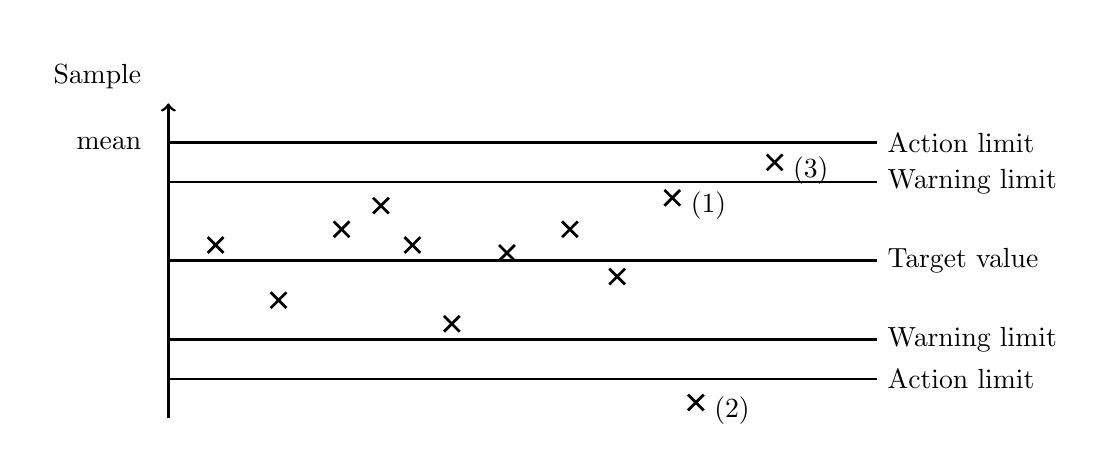
\begin{tikzpicture}
        \draw[->, line width=1] (1, 1) -- (1, 5) node[left]{
            \begin{tabular}{r} Sample \\ mean \end{tabular}
        };
        \draw[line width=1] (1, 4.5) -- (10, 4.5) node[right]{Action limit};
        \draw[line width=1] (1, 4) -- (10, 4) node[right]{Warning limit};
        \draw[line width=1] (1, 3) -- (10, 3) node[right]{Target value};
        \draw[line width=1] (1, 2) -- (10, 2) node[right]{Warning limit};
        \draw[line width=1] (1, 1.5) -- (10, 1.5) node[right]{Action limit};
        \xpoint{1.6}{3.2}
        \xpoint{2.4}{2.5}
        \xpoint{3.2}{3.4}
        \xpoint{3.7}{3.7}
        \xpoint{4.1}{3.2}
        \xpoint{4.6}{2.2}
        \xpoint{5.3}{3.1}
        \xpoint{6.1}{3.4}
        \xpoint{6.7}{2.8}

        \xpointn{7.4}{3.8}{(1)}
        \xpointn{7.7}{1.2}{(2)}
        \xpointn{8.7}{4.25}{(3)}
        \end{tikzpicture}
        \end{center}

        \begin{center}
        \begin{tabularx}{\textwidth}{l|X}
        Event & Action \\
        \hline
        (1) Sample mean is between warning limits & No action \\
        (2) Sample mean outside action limits & Take action \\
        (3) Sample mean between warning and action limits & Take another sample immediently, if the new sample mean is outside warning limits take action \\
        \end{tabularx}
        \end{center}

        \noindent
        To set the limits of a control chart a large sample (when the process is nominal) is taken, known as a proccess capability study. Then find the standard deviation $\sigma$, the size of the continous samples $n$ and the critical values (normaly 95\% and 99.8\%). With this data the confidence itervals for the warning and action limits can be found.

        \begin{example}
        {
            A company manufactures panels for use in making baths. The panels have a target width of 700mm. When a production is satisfactory the widths are normally distributed with a standard deviation of 2mm. Production is to be controlled by taking a regualar sample of 5 panels.
        }

        \begin{step}{Calculate the warning and action limits for a control chart}
        \begin{align*}
        \text{warning limits} &= 700 \pm 1.96 \times \frac{2}{\sqrt{5}}\\
        &= (698.247, 701.753)\\
        &= (698.2, 701.8)
        \end{align*}
        \begin{align*}
        \text{action limits} &= 700 \pm 3.09 \times \frac{2}{\sqrt{5}}\\
        &= (697.236, 702.764) \\
        &= (697.2, 702.8)
        \end{align*}
        \end{step}

        \begin{step}{What action would you take for the following sample $701.2, 698.2, 704.4, 699.4, 695.5$}
        $\bar{x}$ = 699.7\\
        Mean is within warning limits so no action taken.
        \end{step}

        \begin{step}{What action would you take for the following sample $700.2, 697.5, 695.1, 696.0, 698.9$}
        $\bar{x}$ = 697.5\\
        Mean is between warning limit and action limit so another sample should be taken immediently, it it is outside of the warning limits action should be taken.
        \end{step}

        \begin{step}{What action would you take for the following sample $699.5, 707.1, 704.9, 703.9, 706.4$}
        $\bar{x}$ = 704.4\\
        Mean is outside action limits so take action immediently.
        \end{step}

        \end{example}

        \paragraph{Target values} Sometimes the target value is not defined/unattainable, it this case a large samples sample mean could be used. In the case were a warning that a process is doint better than expected (i.e. the strength of a iron casting is stronger than expected) an invistigation should be ran to see how the improvement can be maintained.
    
    \newpage
    \subsubsection{Control of varibility}
        Within a sample their may be high varibility but a normal looking mean, to detect these events we can use a chart for range or a chart for standard deviation. To get the upper and lower limits for these charts multiply the short-term standard deviation by the appropiate value of D/E on table 12 (Control charts for varibility). Standard deviation charts have a better chance to detect a change in varibility with the same rate of false positives as a range chart, however the range is simpler to calculate.

        \begin{example}
        {
            The same company (as in the previous example) wants to control varibility.
        }

        \begin{step}{Calculate upper and lower warning limits for a standard deviation chart}
        \begin{itemize}
        \item Upper action limit $2.15 \times 2 = 4.30$
        \item Upper warning limit $1.67 \times 2 = 3.34$
        \item Lower warning limit $0.35 \times 2 = 0.70$
        \item Lower action limit $0.15 \times 2 = 0.30$
        \end{itemize}
        \end{step}

        \begin{step}{What action would you take for the following sample $701.2, 698.2, 704.4, 699.4, 695.5$}
        $\sigma = 3.328$\\
        Standard deviation is within warning limits so no action taken.
        \end{step}
        
        \begin{step}{What action would you take for the following sample $700.2, 697.5, 695.1, 696.0, 698.9$}
        $\sigma = 2.077$\\
        Standard deviation is within warning limits so no action taken.
        \end{step}

        \begin{step}{What action would you take for the following sample $699.5, 707.1, 704.9, 703.9, 706.4$}
        $\sigma = 2.991$\\
        Standard deviation is within warning limits so no action taken.
        \end{step}

        \end{example}
    
    \newpage
    \subsubsection{Estimating short-test standard deviation}
        Sometimes its not possible to collect a large sample to find the target value, instead we can estimate it from the range of several samples. Find the range of all the samples then find the mean range. Multiply this value by the suitable b value from table 12 to find an estimate for the standard deviation. Alternativly the b value can be applied to all the ranges and the mean of those values can be used.

        \begin{example}
        {
            9 samples of size 5 from a production process have ranges of:
            $$
            2.3, 2.9, 1.8, 3.4, 2.0, 3.6, 2.9, 2.1, 1.1
            $$
            Estimate the standard deviation of the process
        }

        \begin{step}{}
            \begin{align*}
            \text{mean range} &= \frac{2.3+2.9+1.8+3.4+2.0+3.6+2.9+2.1+1.1}{9}\\
            &= \frac{16.5}{9}\\
            &= 1.8333\\
            \\
            1.8333 \times 0.4299 &= 0.7881\\
            &= 0.788\\
            \end{align*}
        \end{step}

        \end{example}

    \newpage
    \subsubsection{Tolerance limits}
        Many processes have limits which the product \textit{must} conform to. For example drugs imagine a drug with a tollerance of 4.9 to 5.1 (for potency) with a target value of 5.0. Its esimated standard deviation was 0.063 which gives the following upper and lower limits.
        \begin{align*}
        z_1 &= \frac{4.9-5.0}{0.063}\\
        &= -1.587\\
        \\
        z_2 &= \frac{5.1-5.0}{0.063}\\
        &= 1.587
        \end{align*}
        which means $1 - 0.887 = 11.3\%$ of the drugs would be outside the tollerance limits.\\
        \\
        If a process's tollerance width exceeds 6 standard deviations the process can be said to meet the tolernaces consitently, given that the mean is kept on target. The drug had a tollerance width of $\displaystyle\frac{0.51 - 0.49}{0.063} = 3.2$ standard deviations.

        \begin{example}
        {
            A biscuit factory produces cream crackers. Packets are sampled at hourly intervals and the weight, in grams, of the contents measured. The results below are from seven samples each of size 5, taken at a time when production was thought to be satisfactory. The target value is 210g.

            \begin{center}
            \begin{tabular}{c|c|c|c|c|c|c}
            \multicolumn{7}{c}{Sample}\\
            1         & 2         & 3         & 4         & 5         & 6         & 7         \\
            \hline
            $209.0$   & $214.5$   & $204.5$   & $217.5$   & $211.0$   & $224.0$   & $210.0$   \\
            $211.0$   & $210.0$   & $209.0$   & $216.0$   & $198.0$   & $220.0$   & $208.0$   \\
            $213.5$   & $212.0$   & $198.5$   & $217.0$   & $209.5$   & $224.0$   & $210.0$   \\
            $205.0$   & $203.5$   & $203.0$   & $214.0$   & $213.5$   & $218.5$   & $220.0$   \\
            $210.0$   & $214.0$   & $213.5$   & $209.5$   & $213.5$   & $210.0$   & $211.0$   \\
            \end{tabular}
            \end{center}
        }

        \begin{step}{Estimate the standard deviation of the process}
        $$\text{ranges} = 8.5, 11, 15, 8, 15.5, 14, 12$$
        $$\text{mean range} = 12$$
        \begin{align*}
        \sigma &= b \times 12 \\
        &= 0.4299 \times 12 \\
        &= 5.1588 \\
        &= 5.16
        \end{align*}
        \end{step}

        \begin{step}{The tollerance for this process is 200g to 220g, comment on the the ability to meet these tollerances}
        The tollerance width is $\displaystyle\frac{220 - 200}{5.16} = 3.88$ standard deviations wide which is bellow the 6 standard deviations we would expect for a process to meet tollerances consistently.
        \end{step}

        \end{example}

    \newpage
    \subsubsection{Control of proportion}
        Control charts may also be used when items are classified as conforming/non-conforming (instead of by weight or height etc). Consider a production line were samples were taken when the production was thought to be satisfactory. With a sample size of 100, the following are the number of non-conforming items in each sample:
        $$
        10, 13, 12, 19, 8, 14, 17, 16, 10, 18, 9, 16
        $$
        The total number of non-conforming items are 162, so the estimate for the proportion of non-conforming items would be $\hat{p} = \dfrac{162}{1000} = 0.135$. Given $\hat{p}$ and sample size $n$, we can find the confidence interval for proportion hence we can find the action and warning limits

        \begin{example}
        {
            To control a process producing components for washing machines 75 components are tested every hour and the number of non-conforming components are recorded. The numbers recorded when production was regarded as satisfactory were:
            $$
            6, 16, 12, 9, 14, 19, 7, 13
            $$
        }

        \begin{step}{Find the warning and action limits for a control chart of proportion}
        \begin{align*}
        p &= \frac{6 + 16 + 12 + 9 + 14 + 19 + 7 + 13}{75 * 8}\\
        &= \frac{96}{600}\\
        &= 0.16
        \end{align*}

        \begin{align*}
        \text{action limits} &= 0.16 \pm 3.09 \times \sqrt{\frac{0.16 \times (1 - 0.16)}{75}} \\ 
        &= (0.0292, 0.2908)\\
        \text{warning limits} &= 0.16 \pm 1.96 \times \sqrt{\frac{0.16 \times (1 - 0.16)}{75}} \\
        &= (0.0770, 0.2430)
        \end{align*}
        \end{step}

        \begin{step}{What action would be taken if the next sample was 27}
        $\dfrac{27}{75} = 0.36$ which is outside the action limits so take action.
        \end{step}

        \begin{step}{What action would be taken if the next sample was 15}
        $\dfrac{15}{75} = 0.2$ which is insied the warning limits so no action is taken.
        \end{step}

        \begin{step}{What action would be taken if the next sample was 3}
        $\dfrac{3}{75} = 0.04$ is bellow the warning limit so investigate how this low rate of non-conforming items may be maintained.
        \end{step}

        \end{example}


\newpage
\section{Acceptance Sampling}

    \paragraph{Acceptance Sampling}
    The process of deciding if a large batch of simular items is acceptable by testing a small amount of them.

    \paragraph{Acceptance sampling by attributes} 
    Each item is classified as conforming or non-conforming, if the sample contains to many non-conforming items the batch is rejected.

    \paragraph{Operating characteristic}
    A graph of probabilty of acceptance against proportion of non-conforming in the batch. Providing the sample size if small compared to the batch this will follow a binomial distribution.\\
    \\
    An example of an acceptance sampling plan is to reject a sample (of size 50) if their are more than 2 non-conforming items. This plan would be denoted as:
    $$n = 50, r = 3$$
    or
    $$n = 50, a = 2$$
    where $r$ is reject when $>=$ the value, and $a$ is accept when $<=$ the value, and $n$ is the sample size.\\
    \\
    For any sampling play their is always the risk or rejecting a good batch (Type I error) or accepting a bad batch (Type II error). An ideal sampling play has the large probabilty of accepting a good batch, and a small probabilty of accepting a bad batch.

    \begin{example}
    {
        An acceptance sampling scheme consists of a sample of $m$ components being taken from a batch. The atch is rejected if $r$ or more non-conforming components are found in the sample, otherwise it is accepted. 
    }

    \begin{step}{If $n = 30$ and $r = 2$, find the probabilty of accepting a batch containing $1\%, 2\%, 4\%, 7\%, 10\%, 15\%, 20\%$ non-conforming components}
    \begin{center}
    \begin{tabular}{c|c|c}
    Percentage & Distribution & Probabilty \\
    \hline
    1\%  & $X \sim B(30, 0.01)$ & 0.964 \\
    2\%  & $X \sim B(30, 0.02)$ & 0.879 \\
    4\%  & $X \sim B(30, 0.04)$ & 0.661 \\
    7\%  & $X \sim B(30, 0.07)$ & 0.369 \\
    10\% & $X \sim B(30, 0.10)$ & 0.184 \\
    15\% & $X \sim B(30, 0.15)$ & 0.048 \\
    20\% & $X \sim B(30, 0.20)$ & 0.010
    \end{tabular}
    \end{center}
    \end{step}

    \begin{step}{Draw the operating characteristic}
    
    \begin{center}
    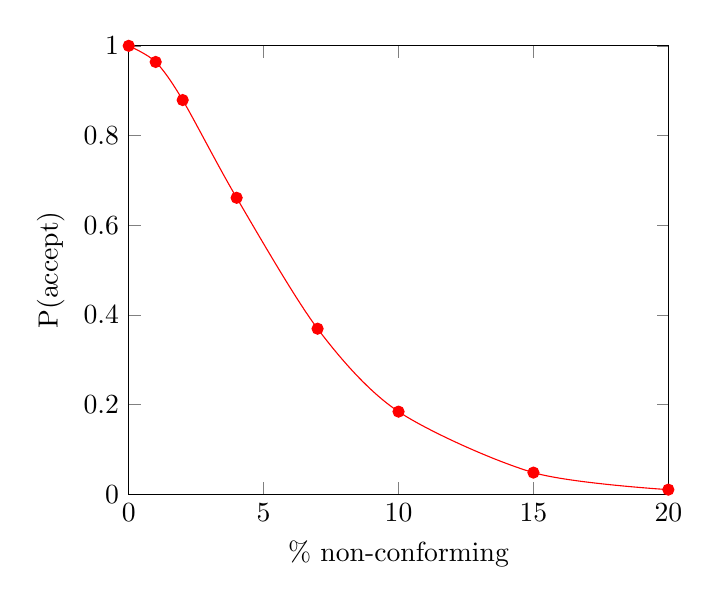
\begin{tikzpicture}
    \begin{axis}[
        xlabel={\% non-conforming},
        ylabel={P(accept)},
        xmin=0, xmax=20,
        ymin=0, ymax=1,
    ]
    \addplot[smooth,color=red,mark=*]coordinates {
    (0, 1)(1,0.964)(2,0.879)(4,0.661)(7,0.369)(10,0.184)(15,0.048)(20,0.010)
    };
    \end{axis}
    \end{tikzpicture}
    \end{center}

    \end{step}
    \end{example}

    \subsection{Accepting a plan}
    The operating characteristic summerizes the implications of a plan however it does not decide what plan should be used. If the sample size and acceptable level of risk is specified it is possible to derive a plan. For example say a manafacture wants their to be at least a 95\% chance of accepting a batch with 1\% non-conforming itesm where $n = 50$.

    \begin{center}
    \begin{tabular}{c|c}
    $r$ & $P(X < r-1)$ \\
    \hline
    1 & $0.605$ \\
    2 & $0.911$ \\
    3 & $0.986$ \\
    4 & $0.998$ \\
    \end{tabular}
    \end{center}

    \noindent
    So when $r = 1$ the chance of accepting a batch with 1\% of non-conforming items is 60.5\% which is less than the required 95\%. Plans were $r > 2$ all fit the requirement, however we also want to minimize the chance of accepting a bad batch so the manafacture should use $r = 3$.

    \begin{example}
    {
        An manafacturer will accept a risk of not more than 10\% of a batch of items containing 2\% non-conforming begin rejected. A decision is to be made by examining a sample of 50 items.
    }

    \begin{step}{Find an appropiate decision procedure}
    $$X \sim B(50, 0.02)$$

    \begin{center}
    \begin{tabular}{c|c}
    $r$ & $1 - P(X < r-1)$ \\
    \hline
    1 & $0.636$ \\
    2 & $0.264$ \\
    3 & $0.078$ \\
    \end{tabular}
    \end{center}

    $$r = 3$$
    \end{step}

    \end{example}

    \subsection{Double sampling plans}
    With a single sample it is very likely to detect a very good/bad batch however for a more intermediate batch it makes a large sample is required for more accuracy.
    $$n = 30; a = 1, r = 3$$
    $$n = 30; a = 4, r = 5$$
    This is an example of a double sampling plan, If the first sample has exactly 2 non-conforming items a second sample is taken else it is accepted/rejected.

    \subsection{Acceptance sampling by variable}
    Acceptance sampling can be carried out by measuring a varible, say the strength of each item. If the mean of theses measurements $\bar{x}$ is above a threshold $k$ then the batch is accepted, else it is rejected. The operating characteristic for a test by varible would be the mean of the measurement against the probabilty of accepting the batch. Its a reasonable to assume the normal distribution since we are conserned with the mean of a large sample.

    \begin{example}
    {
        A batch of bricks are tested for strength which follows a normal distribution with a standard deviation of 5.5. A batch is accepted if the mean of five bricks is greated than 51.
    }

    \begin{step}{Draw the operating characteristic}
    The standard deviation of the sample mean will be $\dfrac{5.5}{\sqrt{5}} = 2.46$. Since most data is within 3 standard deviation (on both sides) we will use a range of 44-58.
    
    \begin{center}
    \begin{tabular}{c|c|c}
    $\mu$ & $\dfrac{51-\mu}{\dfrac{5.5}{\sqrt{5}}}$ & $P(\text{accept})$ \\
    \hline
    44 & 2.846 & 0.002 \\ 
    46 & 2.033 & 0.021 \\
    48 & 1.220 & 0.111 \\
    50 & 0.407 & 0.342 \\
    52 & -0.407 & 0.658 \\
    54 & -1.220 & 0.889 \\
    56 & -2.033 & 0.979 \\
    58 & -2.846 & 0.998 \\
    \end{tabular}
    \end{center}
    
    \begin{center}
    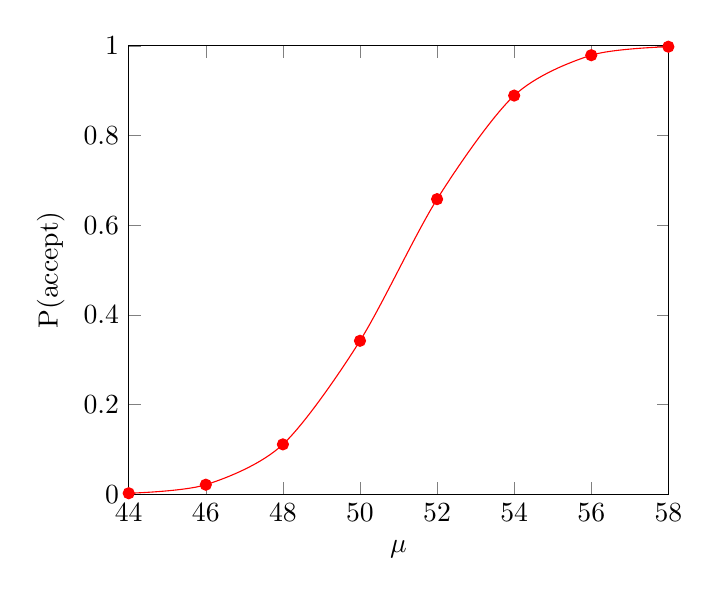
\begin{tikzpicture}
    \begin{axis}[
        xlabel={$\mu$},
        ylabel={P(accept)},
        xmin=44, xmax=58,
        ymin=0, ymax=1,
    ]
    \addplot[smooth,color=red,mark=*]coordinates {
    (44, 0.002)(46, 0.021)(48, 0.111)(50, 0.342)(52, 0.658)(54, 0.889)(56, 0.979)(58, 0.998)
    };
    \end{axis}
    \end{tikzpicture}
    \end{center}

    \end{step}
    
    \begin{step}{The customer requires the probability of accepting a batch with a mean strength of 47 or less should be less than 10\%, would the customer be satisfied with the curren acceptance sampling}
    47 is approximatly 0.05 or 5\% (from the operating characteristic) so the customer would be satisfied.
    \end{step}

    \begin{step}{Whats the smallest value for $k$ which would meet the customers requirements if $n = 6$}
    \begin{align*}
    \frac{k - 47}{\dfrac{5.5}{\sqrt{5}}} &> 1.2816 \\
    k - 47 &> 2.8776 \\
    k &> 49.8776
    \end{align*}
    $$k = 49.9$$
    \end{step}

    \end{example}